% =============================================================================
% PRL variant of the troposwhere manuscript (K=5).
% Reformatted from the Nature-Comp-Sci article-class version
% (preserved in main_natcomp_backup.tex) into REVTeX 4.2 / Physical Review
% Letters format: two-column reprint layout, numeric APS citations
% (apsrev4-2.bst), PRL title/abstract block.
%
% CONVERSION STATUS (pass 1 = reformat; content preserved, not yet cut to
% the PRL length limit ~3750 words / 4 pages):
%   [x] REVTeX 4.2 preamble, prl option, two-column reprint
%   [x] Numeric \cite throughout (was authoryear \citep/\citet)
%   [x] Title / author / affiliation / abstract block
%   [x] Body ported (intro + results + discussion)
%   [x] Methods kept at end (candidate for Supplemental Material / End Matter)
%   [ ] Cut to PRL length (pass 2)
%   [ ] Split heavy Methods -> Supplemental Material (pass 2)
%   [ ] Verify author affiliations (marked TODO below)
% =============================================================================
% Review layout: reprint class (compact title block -> abstract on page 1,
% no empty title page), but the body is forced to a single wide column via
% \onecolumngrid after \maketitle so that line numbers sit cleanly in the
% left margin without the two-column gutter overlap. For the final
% journal-look two-column preview, comment out the \onecolumngrid line below.
\documentclass[
    aps,
    prl,
    reprint,
    superscriptaddress,
    amsmath,amssymb,
    floatfix,
    nofootinbib
]{revtex4-2}

% ── Figures, math, typography ──────────────────────────────────────────
\usepackage{graphicx}
\usepackage{bm}
\usepackage{xcolor}
\usepackage[colorlinks=true,allcolors=blue!50!black,citecolor=blue!50!black]{hyperref}
\usepackage{xr-hyper}                             % cross-refs to Supplemental Material labels
\externaldocument[S]{supplementary}                  % reads supplementary.aux (build SM first)
\usepackage{lineno}                               % line numbers (clean in single-column preprint)
\usepackage{setspace}                             % wider line spacing for the review copy
% \linenumbers is issued after \maketitle (below) to avoid a lineno/REVTeX
% interaction that pushes the abstract onto a blank second page.

\graphicspath{{./}{figures/}{SI_figures/}{img/}}

\begin{document}

\title{A temporally-constrained latent space reveals \\ 
the stochastic dynamics of convective organization}

\author{Sophie Abramian}
\affiliation{Department of Earth and Environmental Engineering, Columbia University, New York, NY, USA}

\author{Olivier Pauluis}
\affiliation{Courant Institute of Mathematical Sciences, New York University, New York, NY, USA}

\author{L. Ruby Leung}
\affiliation{Atmospheric Sciences and Global Change Division, Pacific Northwest National Laboratory, Richland, WA, USA}


\author{Pierre Gentine}
\affiliation{Department of Earth and Environmental Engineering, Columbia University, New York, NY, USA}




\date{\today}

\begin{abstract}
Atmospheric convection is intrinsically stochastic: under identical large-scale forcing, storms can follow widely different life cycles. We introduce an unsupervised framework that learns a low-dimensional representation of cloud-resolving squall-line simulations by constraining the latent space to evolve according to a linear stochastic operator. The learned representation partitions convection into five physically interpretable states whose transitions define a Markov chain. Its spectrum reveals a dominant slow mode separating organized from unorganized convection and governing the system's life cycle. The remaining departures from Markovianity are partly explained by cold pools, identifying a physical source of memory absent from the reduced description. The framework provides a physically interpretable stochastic coarse-graining of convection and offers an alternative to existing multi-cloud parameterizations.
\end{abstract}

\maketitle

% ── Introduction (no heading, PRL Letter style) ────────────────────────
Discovering interpretable, low-dimensional representations of high-dimensional stochastic systems is a foundational challenge across the physical sciences. Deep convection is a prime example: deep convective systems---organized cloud structures larger and longer-lived than individual cells---dominate the tropical water and energy cycle \cite{houze2004mesoscale, chakraborty2023overview}; the largest contribute over 50\% of tropical precipitation and a disproportionate share of extremes \cite{roca2020extreme, feng2024mesoscale, feng2023mesoscale}.

In climate models they occur below the grid scale and must be parameterized, a persistent source of uncertainty under warming \cite{yang2023impact, bolot2025no}. The difficulty is that a convective system is high-dimensional: compressing it into a few prognostic variables without discarding what matters is hard.

Compounding this, under \emph{fixed} large-scale forcing the convective response is not a single outcome but a broad distribution of storm evolutions \cite{abramian2025key, feng2025mesoscale, hu2020observed, fiolleau2024database}---an \emph{internal} variability intrinsic to convection. Capturing it requires a low-dimensional reduced description faithful to the dynamics.

Stochastic multi-cloud models \cite{khouider2006multicloud, majda2008stochastic, khouider2010stochastic} offer such a reduction, but one whose states are prescribed \emph{a priori}: a lattice of sites, each in one of a few hand-chosen cloud states---clear sky, shallow, congestus, or deep---whose area fractions evolve by a Markov chain. This captures the changing cloud cover but not the vertical mass-flux profiles that also govern extreme precipitation \cite{MullerYukari19, singh2012upward, abramian2023extreme, wang2022convective, li2025bimodal}.

Koopman operator theory \cite{koopman1931hamiltonian, brunton2021modern} offers a principled alternative. Instead of the state $\mathbf{x}_t$ of a high-dimensional nonlinear system, one follows \emph{observables} $g(\mathbf{x})$ that recast it in new coordinates; the operator advancing them---$\mathcal{K}$, the Koopman operator, defined by $(\mathcal{K}g)(\mathbf{x}_t) = g(\mathbf{x}_{t+1})$---is linear by construction, whatever the nonlinear dynamics. The challenge is then not to resolve the nonlinear evolution but to find an observable that simplifies it while retaining most of the system's information. Such an observable is generally infinite-dimensional \cite{brunton2021modern}---the long-standing obstacle. Only recently have machine-learning encoder--decoder architectures \cite{lusch2018deep, nathaniel2026generative} overcome it, learning from data the best finite-dimensional observable and its linear operator.

We depart from existing Koopman autoencoders in two ways. First, we start from a physically reduced representation, casting the flow in isentropic coordinates \cite{pauluis2013isentropic}---a thermodynamically consistent reduction that filters reversible adiabatic motions---rather than raw three-dimensional fields. Second, rather than enforcing \emph{deterministic} linear dynamics, we \emph{partition} the latent space into discrete states by joint clustering \cite{kaiser2014cluster, souza2024representing} and model their transitions \emph{probabilistically}. The result is a Markov chain whose states are discovered from the data rather than prescribed. Though demonstrated on convection, the framework applies to any high-dimensional system needing regime discovery and transition modeling.

We analyze cloud-resolving simulations of squall lines (SAM~\cite{khairoutdinov2003}) under fixed vertical wind shear, in statistical equilibrium with strong internal variability. At each time the three-dimensional vertical mass flux is projected onto height $z$ and moist static energy $h$, yielding a two-dimensional diagram $M(h,z)$ that separates high-$h$ updrafts from the low-$h$ evaporative downdrafts that build cold pools~\cite{pauluis2013isentropic}. Figure~\ref{fig:simu_isentrop} shows three representative snapshots alongside their mass-flux diagrams; this time series is the input to the model.

\begin{figure}[t]
    \centering
    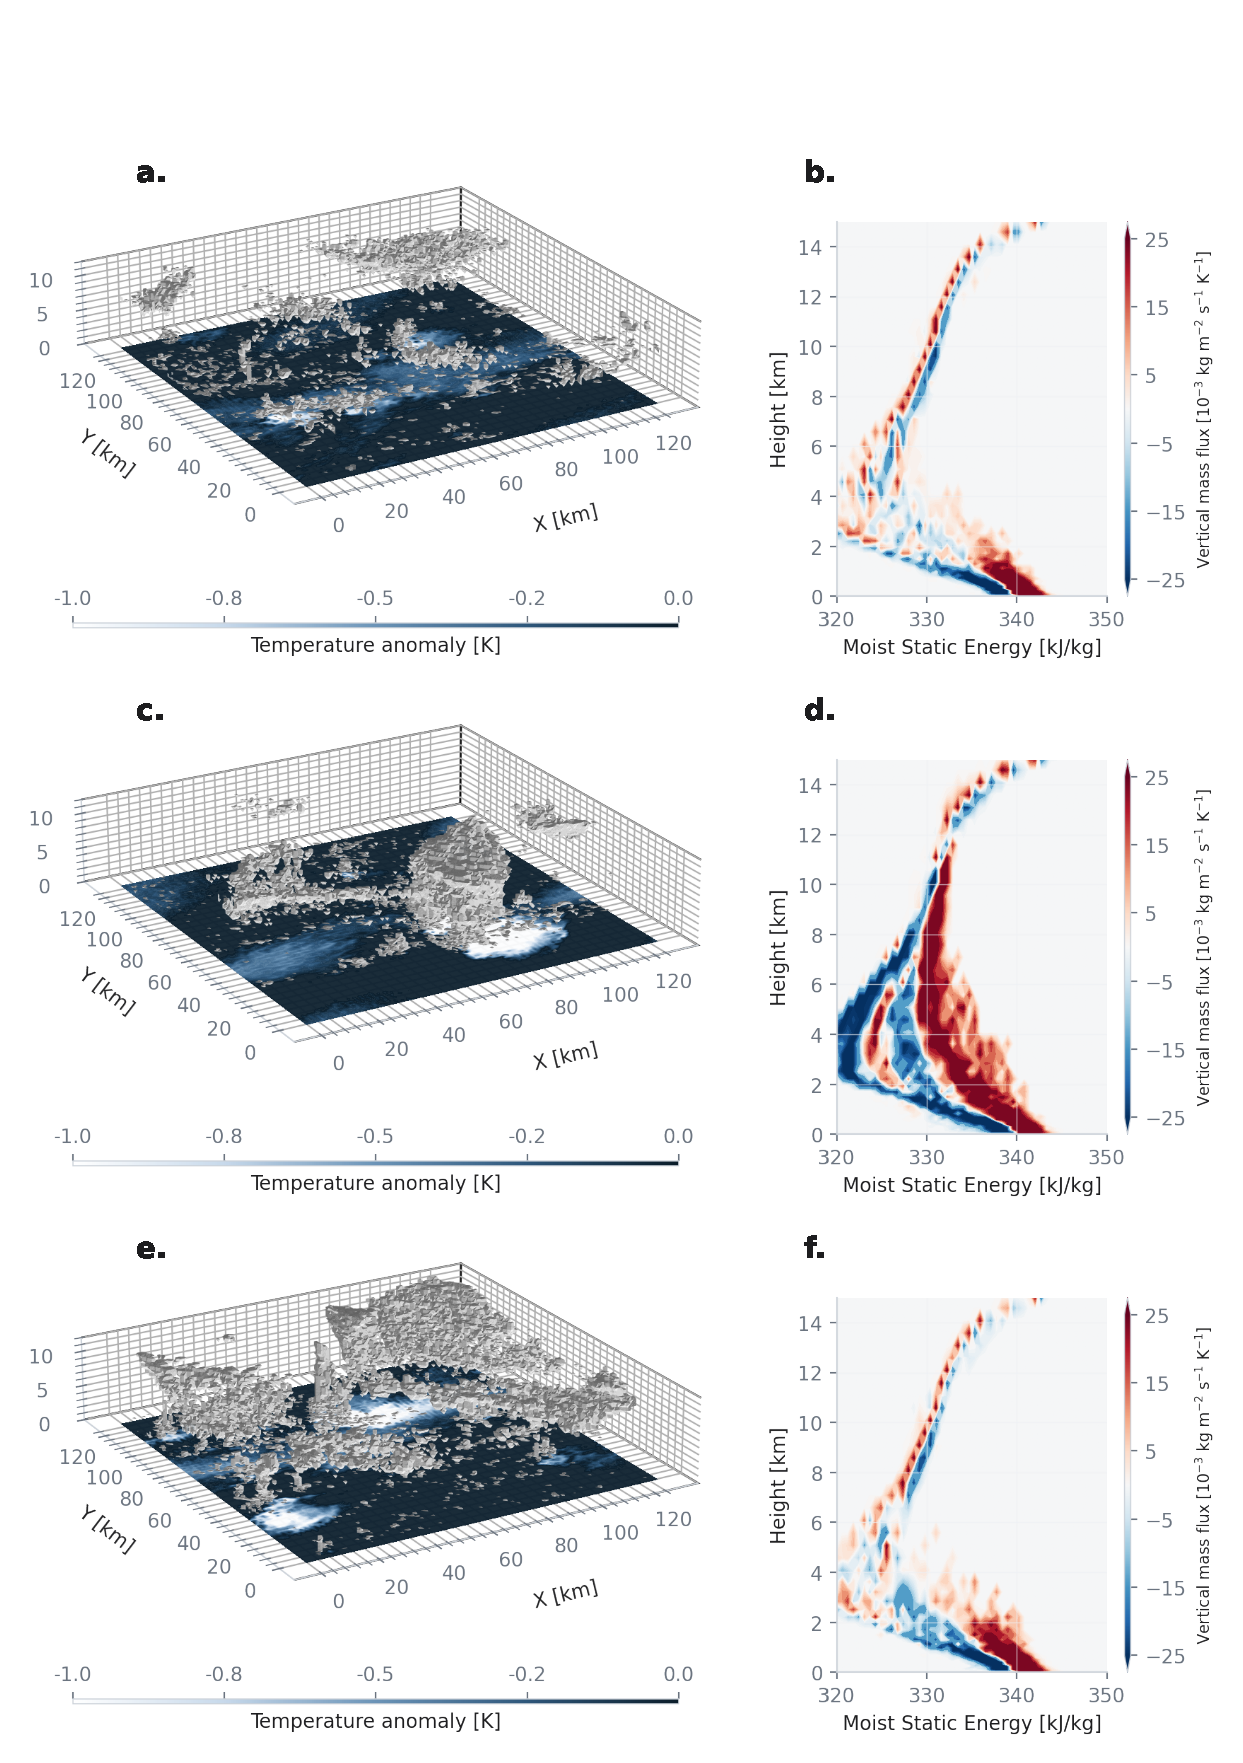
\includegraphics[width=\columnwidth]{fig1_snapshots.pdf}
    \caption{\textbf{Three contrasting snapshots of the convective field.} \textbf{Left (a, c, e):} isovolume of non-precipitating condensate $\mathrm{QN}=0.02$~kg\,kg$^{-1}$ over the surface temperature anomaly; white patches mark cold pools. \textbf{Right (b, d, f):} isentropic mass-flux diagram $M(h,z,t)$, red (blue) for upward (downward) transport. Rows: \textbf{(a--b)} suppressed, \textbf{(c--d)} organized deep, \textbf{(e--f)} unorganized active.}
    \label{fig:simu_isentrop}
\end{figure}

Applied to these simulations, the construction asks: (i)~what mass-flux states a given forcing makes accessible; (ii)~whether their transitions form a Markov chain, and how organized and weakly organized pathways differ; (iii)~where internal feedbacks---cold pools in particular---introduce memory beyond the discrete state. Five interpretable states emerge without supervision, and their transitions form a Markov chain with a slow ($\sim$3\,h) eigenmode alternating two regimes, organized and unorganized; two long-lived states decay more slowly than their Markov prediction, and conditioning on cold-pool intensity closes $\sim$30\% of that gap.

% ── Results ────────────────────────────────────────────────────────────
\section{Construction and physical interpretation of the latent space}

The squall-line evolution is seen through its time series of isentropic mass-flux fields $X_t$. An encoder maps $X_t$ to a Gaussian posterior over a latent vector $\mathbf{z}_t\in\mathbb{R}^8$ (a variational autoencoder with reconstruction and Kullback--Leibler terms); a softmax head turns $\mathbf{z}_t$ into a probability vector $s_t$ over $K=5$ states; and a row-stochastic matrix $\mathbf{T}$ propagates it one step, $s_{t+1}\approx\mathbf{T}\,s_t$. The three are trained jointly on consecutive pairs $(X_t, X_{t+\Delta t})$, so the latent space is at once reconstructive, cluster-separable, and dynamically predictive (Fig.~\ref{fig:model}). A contrastive (Dice) loss on the mass-flux fields prevents state collapse, keeping all five states populated. Full details are in the Supplemental Material.

\begin{figure}[!ht]
    \centering
    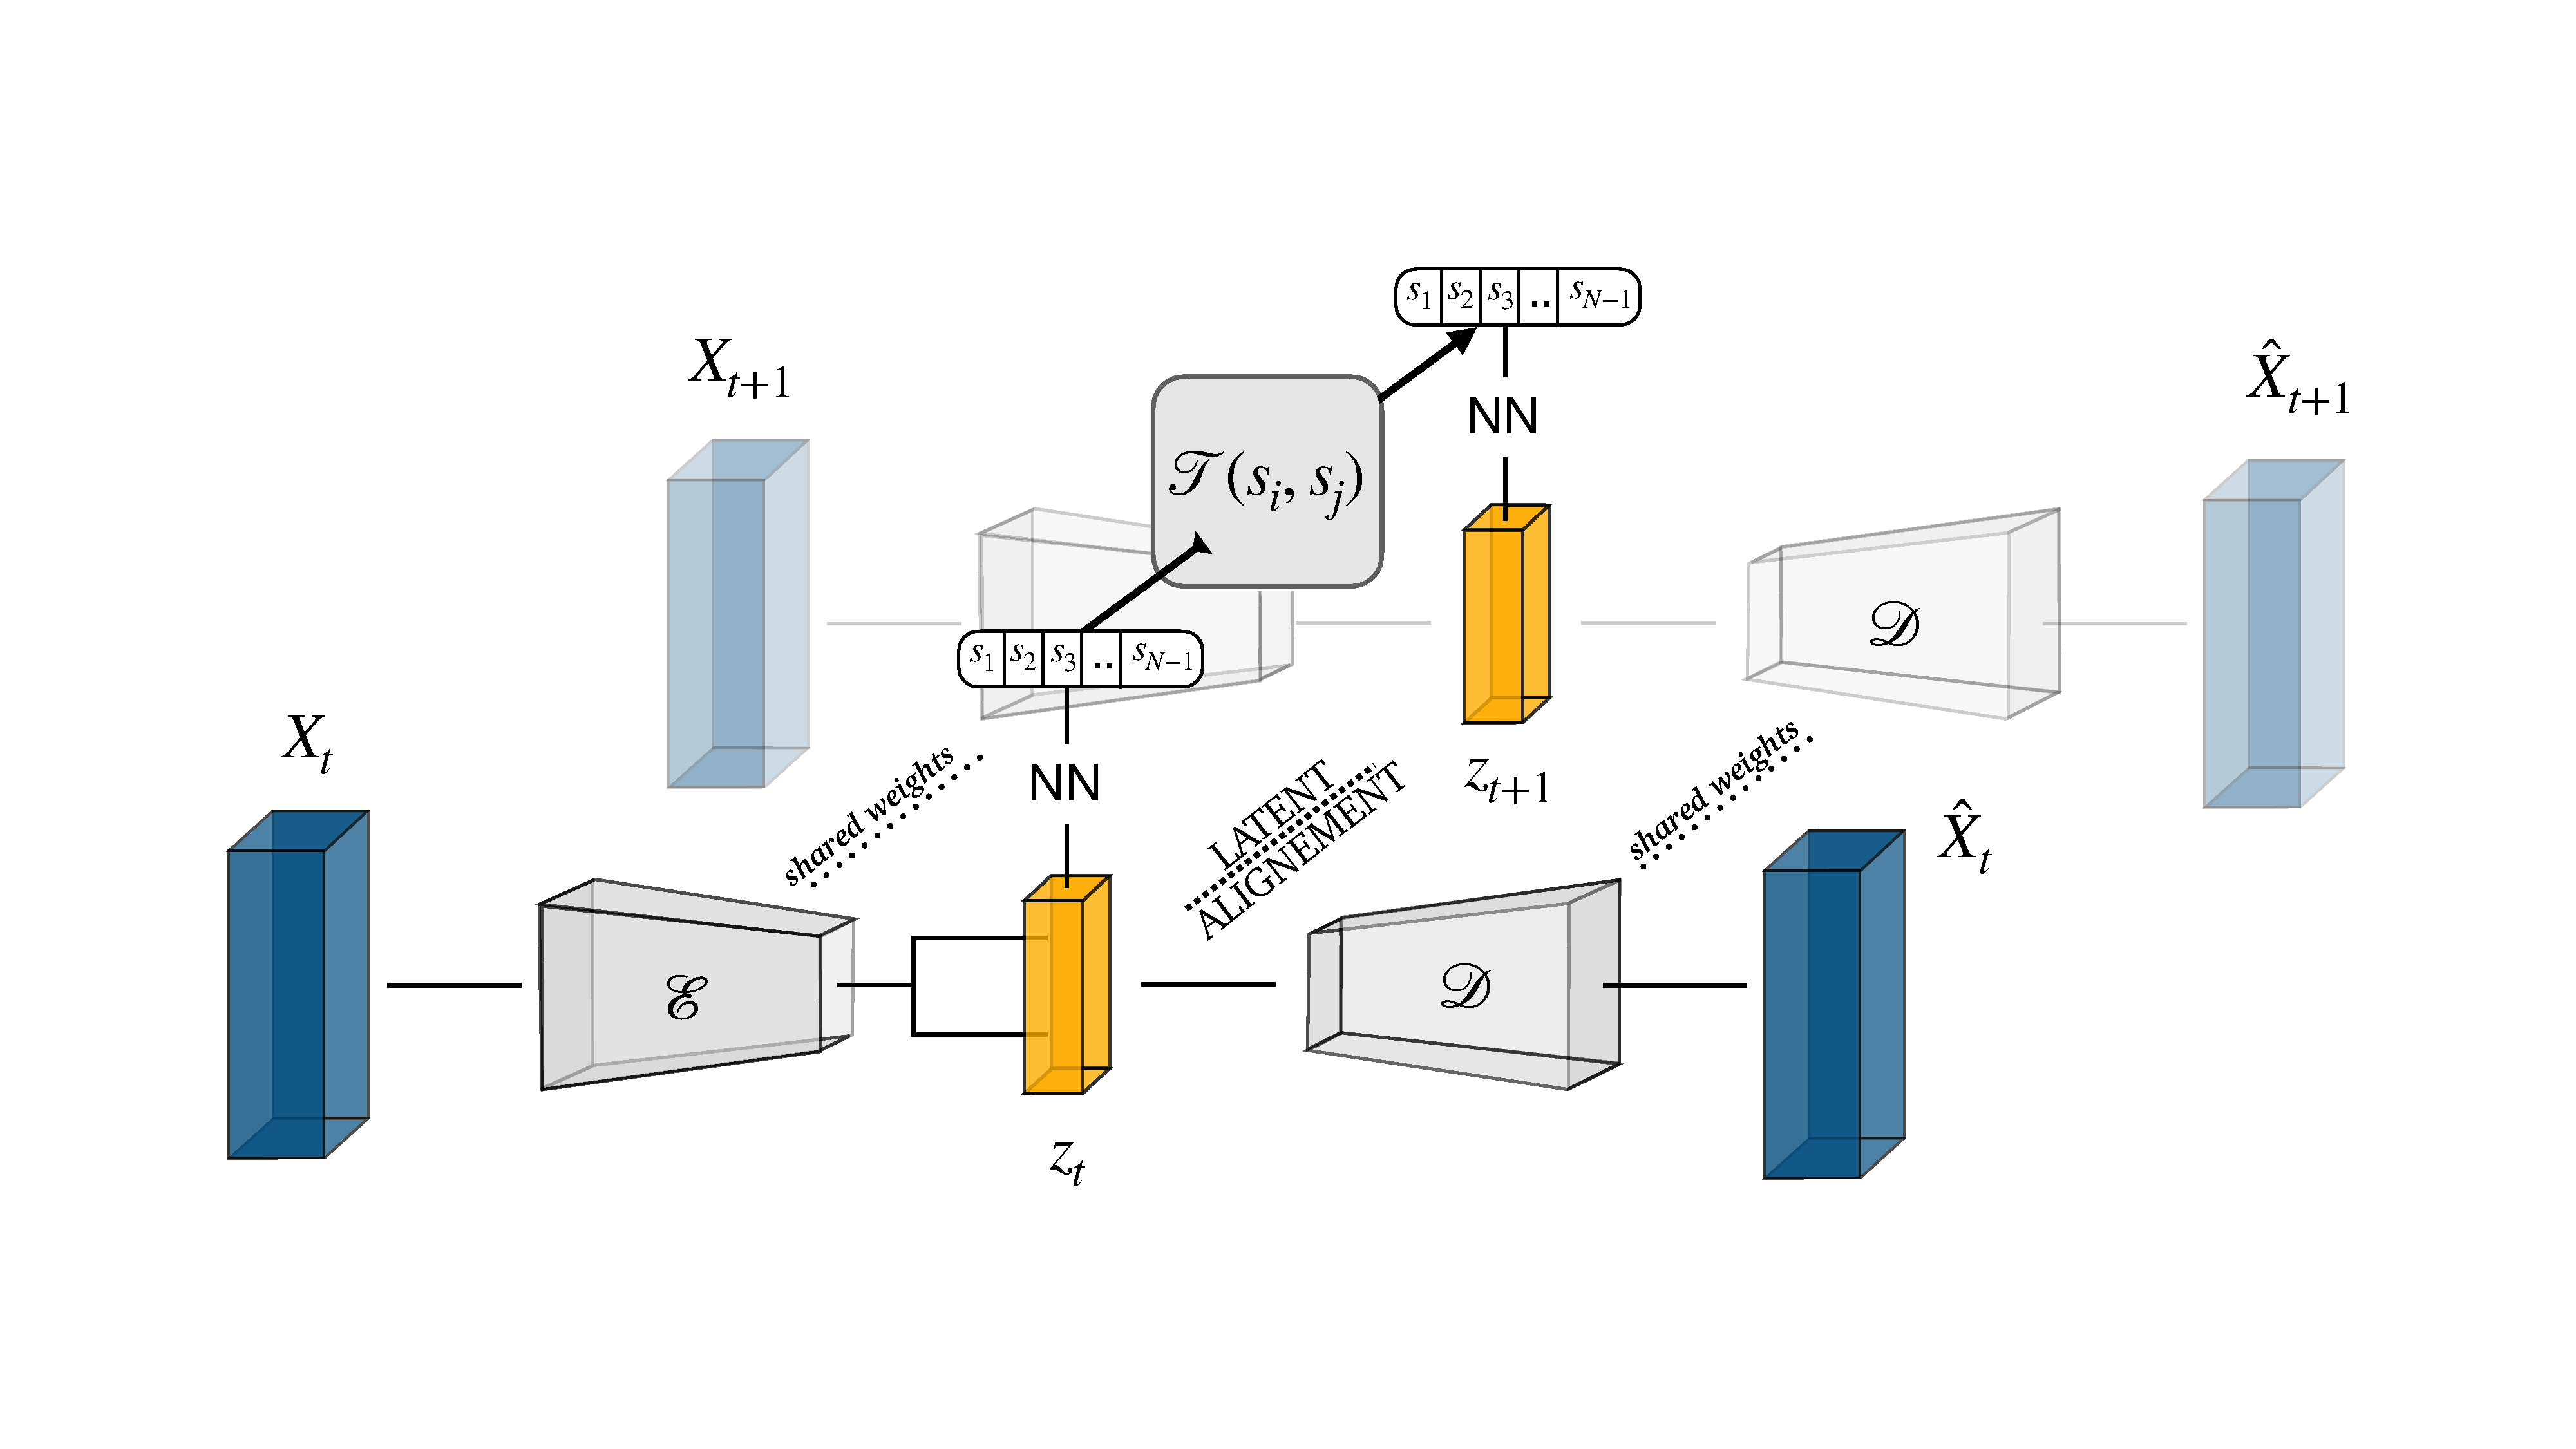
\includegraphics[width=\columnwidth]{model_vae_mc.pdf}
    \caption{\textbf{Model architecture.} A variational autoencoder is coupled to a Markovian state-assignment and transition framework and trained jointly (components defined in the text).}
    \label{fig:model}
\end{figure}

No physical constraint is imposed during training: the VAE is regularized only toward an isotropic Gaussian and states are assigned without reference to any physical diagnostic, so a physically meaningful latent space is not guaranteed. Applying PCA to $\mathbf{z}(t)$, the first two components explain $22\%$ and $17\%$ of the variance (Fig.~\ref{fig:clusters}); a three-dimensional projection (Supplemental Material, Fig.~\ref{Sfig:pca_3d}) shows that states overlapping in 2D separate along higher-order components.

\begin{figure*}[t]
    \centering
    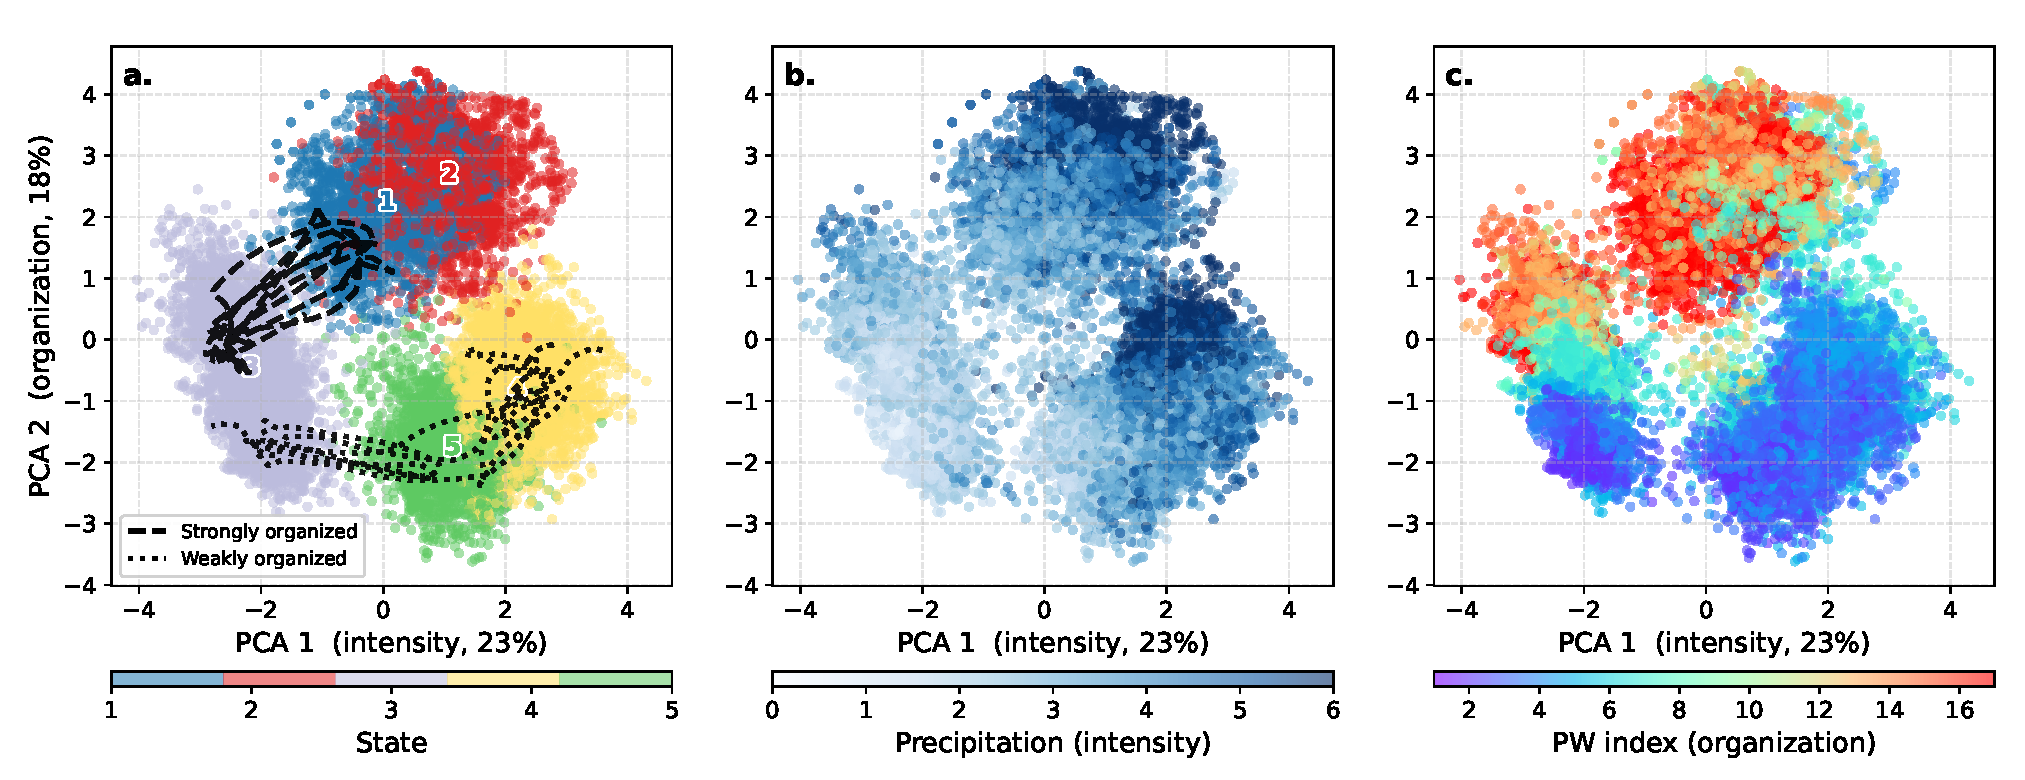
\includegraphics[width=0.98\textwidth]{fig_pca_panels.pdf}
    \caption{\textbf{Latent-space visualization and physical interpretation.} PCA projection of the latent space (each point is one time step), coloured by \textbf{(a)}~state assignment, with two example trajectories over 5~h (dashed: strongly organized; dotted: weakly organized); \textbf{(b)}~domain-mean precipitation, a proxy for convective intensity; and \textbf{(c)}~the variance of precipitable water (the PW index), a proxy for spatial organization (higher values indicate more clustered convection). Joint distributions are given in the Supplemental Material (Fig.~\ref{Sfig:axis_var}).}
    \label{fig:clusters}
\end{figure*}

The dominant latent directions are physically interpretable (Fig.~\ref{fig:clusters}). The first principal component correlates strongly with domain-mean precipitation---convective intensity and life-cycle stage, from suppressed to vigorously precipitating. The second is nearly uncorrelated with precipitation but strongly anticorrelated with the variance of precipitable water, a proxy for spatial organization. Intensity and organization thus emerge as two largely independent axes of the learned representation.

The five states are also dynamically and thermodynamically distinct. Averaging the isentropic mass flux within each state as anomalies from the simulation-wide mean (definitions and full profiles in the End Matter, Figs.~\ref{fig:vertical_profiles} and~\ref{fig:mse_profiles}) shows that the organized-deep and stratiform-like states carry deep, high--moist-static-energy ascent, while the active-unorganized state peaks at lower altitude and lower moist static energy, and the suppressed and shallow-congestus states carry only weak, shallow anomalies. Table~\ref{tab:state_summary} summarizes each state.

\begin{table*}[t]
\centering
\begin{ruledtabular}
\begin{tabular}{c l c p{0.42\textwidth}}
State & Name & $\pi$ (\%) & Physical signature \\
\hline
1 & \emph{Organized deep}     & 12.9 & sustained deep ascent in a moist environment; reduced low-level detrainment; highest precipitable-water variance \\
2 & \emph{Stratiform-like}    & 12.2 & strongly active convection with large upper-tropospheric mass flux, consistent with a mesoscale stratiform region; highest precipitation \\
3 & \emph{Suppressed convection} & 37.0 & weak up- and down-drafts; dry background atmosphere; dominant state \\
4 & \emph{Active unorganized}     & 22.7 & active but unorganized convection, with mass flux peaking at lower altitudes than in the organized regime; drier environment \\
5 & \emph{Shallow congestus}      & 15.2 & suppressed deep convection with residual shallow convective activity; dry environment \\
\end{tabular}
\end{ruledtabular}
\caption{\textbf{Summary of the five latent convective states.} Identities are inferred from the latent-space axes (Fig.~\ref{fig:clusters}) and confirmed by the per-state mass-flux profiles (Figs.~\ref{fig:vertical_profiles} and~\ref{fig:mse_profiles}, End Matter). $\pi_i$ is the stationary probability of state~$i$ [Eq.~\eqref{eq:canon}].}
\label{tab:state_summary}
\end{table*}

\section{Markov transition matrix, eigenmodes, and regimes}

The second output of the model is a Markov transition matrix $\mathbf{T}$, whose elements
\begin{equation}
T_{ij} = \mathbb{P}\left( X_{t+\Delta t} = j \mid X_t = i \right)
\end{equation}
denote the probability of transitioning from state $i$ to state $j$. The resulting transition matrix is shown in Fig.~\ref{fig:markov_matrix}.

\begin{figure*}[t]
    \centering
    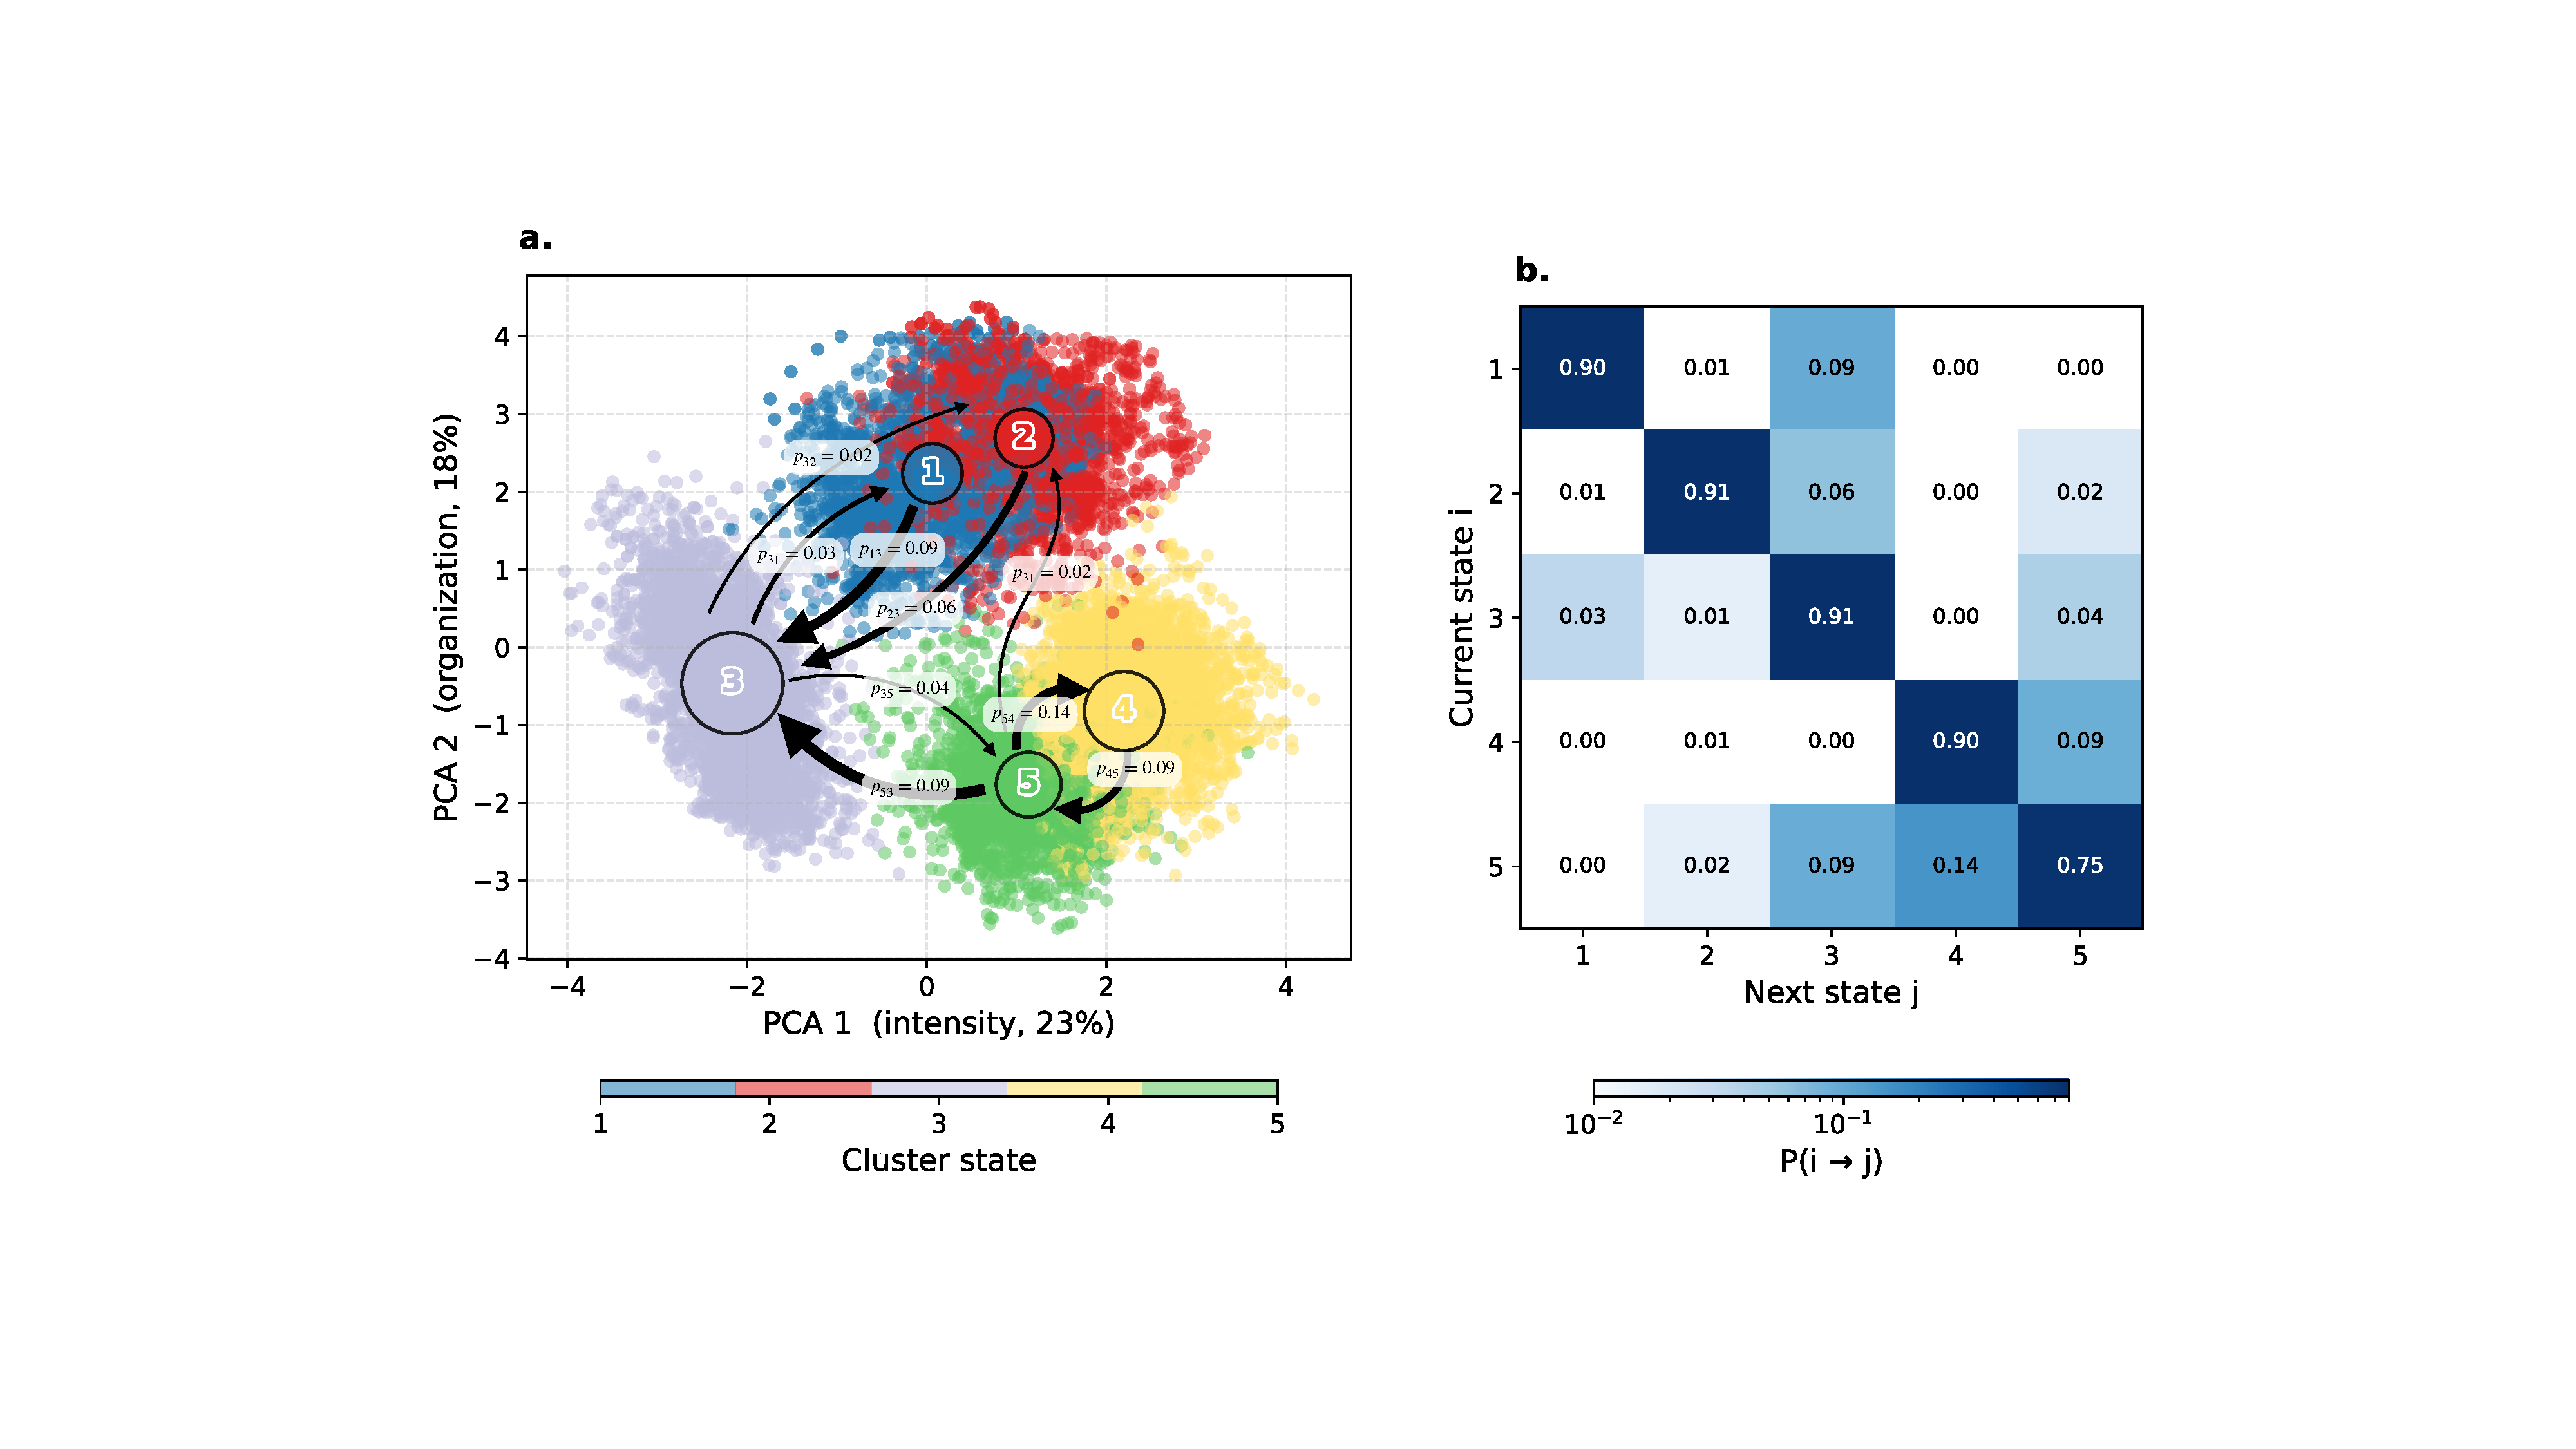
\includegraphics[width=0.92\textwidth]{fig_7_markov_matrix.pdf}
    \caption{\textbf{Markov state dynamics in latent space.} \textbf{(a)} Latent-space visualization; each state node is sized by its stationary probability. \textbf{(b)} Transition matrix for the given shear. Two coupled blocks, separated by state~3, form the organized (states~1--2) and unorganized (states~4--5) regimes.}
    \label{fig:markov_matrix}
\end{figure*}

The matrix $\mathbf{T}$ is strongly diagonally dominant and sparse: the system persists within a state over several steps, with only a few preferred transitions between states.

To characterize the dynamics, we spectrally decompose $\mathbf{T}$. Being stochastic, it admits a unit eigenvalue $\lambda_1=1$ whose right eigenvector $\boldsymbol{\pi}$ satisfies $\mathbf{T}\boldsymbol{\pi}=\boldsymbol{\pi}$, the stationary distribution. We obtain
\begin{equation}
\boldsymbol{\pi} =
\begin{bmatrix}
12.9\% & 12.2\% & 37.0\% & 22.7\% & 15.2\%
\end{bmatrix}.
\label{eq:canon}
\end{equation}

The stationary distribution is dominated by state~3 ($37\%$), the remaining weight spread across the four active states, all sufficiently populated to constrain the transition statistics.

The non-stationary eigenvalues are effectively real ($|\mathrm{Im}(\lambda_k)|<10^{-3}$), so the dominant dynamics are not simple oscillations in state space.

The leading nontrivial eigenvalue is $\lambda_2 \approx 0.94$, a highly persistent mode. The corresponding eigenvector
\begin{equation}
\mathbf{v}_2 =
\begin{bmatrix}
-56\% & -30\% & -25\% & +65\% & +34\%
\end{bmatrix}
\end{equation}
has unit norm (components shown as percentages; the overall sign is arbitrary). A positive $(\mathbf{v}_2)_i$ means state~$i$ is enhanced relative to $\pi_i$ in one phase and suppressed in the other, with amplitude $|(\mathbf{v}_2)_i|$; opposite signs vary in anti-phase.

The components of $\mathbf{v}_2$ split the chain into two opposite-sign groups, $\{1,2\}$ ($-56\%,\,-30\%$) and $\{4,5\}$ ($+65\%,\,+34\%$); state~3 has the smallest amplitude in this mode ($-25\%$). We interpret these two groups as two convective regimes---\emph{organized} ($\{1,2\}$) and \emph{unorganized} ($\{4,5\}$)---that the chain alternates between on the eigenmode decay time $\tau_2 = -\Delta t / \log|\lambda_2| \approx 172\,\mathrm{min}$. State~3 carries the dominant stationary occupancy ($\pi_3=37\%$), and nearly every transition between the other four states passes through it (Fig.~\ref{fig:markov_matrix}b): the chain's intermediate state.

The two regimes differ internally. The unorganized regime is a closed oscillation: states~4 and~5 exchange directly and frequently ($T_{4\to 5}=0.09$, $T_{5\to 4}=0.14$). The organized regime is not: states~1 and~2 do not exchange directly ($T_{1\to 2}=T_{2\to 1}=0.01$) and are separated in time---$200$~min after a state-1 timestep, the probability of being in state~2 is $0.04$, well below the stationary $\pi_2=0.12$. States~1 and~2 therefore appear as independent organized episodes, each returning to state~3 before the next can begin. Individual realizations reflect this (Fig.~\ref{fig:clusters}a): organized intervals show a $3\!\leftrightarrow\!1$ oscillation, unorganized ones the $3\!\leftrightarrow\!5\!\leftrightarrow\!4$ cycle.

The spectrum makes a quantitative prediction: for a true Markov chain, the autocorrelation of each state's occupancy is a sum of exponentials with decay times $\tau_k = -\Delta t / \log|\lambda_k|$.

\section{Markovianity assessment and internal feedbacks}
\label{sec:markov}

We now ask whether the five-state chain is self-contained: whether the state at time $t$ alone determines the distribution at $t+\tau$. Departures identify slow internal processes---moisture memory, cold pools, mesoscale organization---that the partition does not resolve. The question is long-standing: classical parameterizations assume instantaneous quasi-equilibrium \cite{zhang2003convective, bechtold2014representing}, while recent schemes add explicit memory variables \cite{piriou2007approach, gerard2009cloud, mapes2011parameterizing, hwong2023assessing}.

\emph{Indicator autocorrelation.} Defining the occupancy indicator $I_i(t) = \mathbf{1}[X_t = i]$ and its normalized autocorrelation
\begin{equation}
C_i(\tau) =
\frac{\mathbb{E}\!\left[(I_i(t)-\pi_i)(I_i(t+\tau)-\pi_i)\right]}
     {\mathbb{E}\!\left[(I_i(t)-\pi_i)^2\right]},
\end{equation}
a discrete-time Markov chain admits the closed form \cite{souza2024representing}
\begin{equation}
C_i(\tau) \;=\; \frac{T^\tau_{ii} - \pi_i}{1-\pi_i}
\;=\; \sum_{\alpha=2}^K A_\alpha^{(i)}\, \lambda_\alpha^\tau,
\label{eq:autocor}
\end{equation}
a superposition of exponentially decaying modes set by the eigenvalues $\lambda_\alpha$ of $\mathbf{T}$, with amplitudes $A_\alpha^{(i)} = (\mathbf{v}_\alpha)_i (\mathbf{w}_\alpha)_i / (1-\pi_i)$ ($\mathbf{v}_\alpha$, $\mathbf{w}_\alpha$ the right and left eigenvectors; full derivation in the End Matter). Departures from it quantify residual memory not encoded by the partition.

\emph{Memory beyond Markov in the convection-active states.}---In Fig.~\ref{fig:autocorrelation}a, the empirical autocorrelations decrease and fall below $0.2$ within the lag window, in line with the Markov prediction of Eq.~\eqref{eq:autocor}---except for the organized state~1 (blue) and the active-unorganized state~4 (yellow), which stay elevated, well above their predictions; state~3 (suppressed convection) tracks its prediction most closely. This distinction matters: a state can be \emph{sustained} yet still \emph{Markovian} if its diagonal $T_{ii}$ explains the persistence; states~1 and~4 persist \emph{beyond} what $T_{ii}$ predicts, so an internal degree of freedom absent from the partition is keeping them alive.

\emph{Cold pools partly close the gap.}---Cold pools, masses of cold, dense air formed below convective clouds by rain evaporation and a key control on squall-line organization \cite{rotunno1988theory, houze1977structure, tompkins2001coldpools, abramian2022shear}, are a natural carrier of this memory: they outlast the downdrafts that generate them and trigger or suppress convection at their gust fronts \cite{torri2015mechanisms}, sustaining an organized state beyond what the instantaneous partition records. The hypothesis is testable: if cold pools carry the memory, knowing the cold-pool field at the starting time should make the subsequent state~1 dynamics more Markovian. To test this we introduce an indicator that picks out state~1 timesteps with a high cold pool,
\begin{equation}
J_1^\star(t) \;=\; \mathbf{1}\!\left[X_t = 1 \,\text{ and }\, \mathrm{CP}(t) > \mathrm{CP}_\star\right],
\end{equation}
where $\mathrm{CP}(t)$ is a cold-pool index---the total area covered by cold pools at time $t$, normalized by its temporal mean (End Matter, Eq.~\ref{eq:cp_index})---and $\mathrm{CP}_\star$ is its 75th percentile. The cold-pool-conditioned state~1 survival is then the expected state~1 occupancy a lag $\tau$ later, averaged over the timesteps selected by $J_1^\star$:
\begin{equation}
S^{(\mathrm{CP})}_1(\tau) \;=\; \mathbb{E}\!\left[\,I_1(t+\tau) \,\big|\, J_1^\star(t) = 1\,\right].
\end{equation}
We then rescale to autocorrelation form via $C^{(\mathrm{CP})}_1(\tau) = (S^{(\mathrm{CP})}_1(\tau) - \pi_1)/(1-\pi_1)$ for comparison with panel~(a). The condition is applied \emph{only at the starting time}; the trajectory is free thereafter (End Matter). The conditioned curve (Fig.~\ref{fig:autocorrelation}b, dashed) sits between the unconditional empirical curve (solid) and the Markov reference (dotted), closing roughly $30\%$ of the gap at a $200$~min lag: more Markovian, but not fully.

\emph{Cold pools are part---but not all---of the hidden memory.}---The unclosed portion of the gap implicates other slow variables---mesoscale moisture pooling \cite{mapes2011parameterizing}, cloud-cluster geometry \cite{hwong2023assessing}, free-tropospheric humidity---evolving on similar time scales. Two caveats apply: $\mathrm{CP}(t)$ collapses spatial structure into a scalar, and stratifying by it inherits some lifecycle-stage dependence. A definitive identification would require re-training the encoder with explicit cold-pool inputs, left to future work.

\begin{figure*}[t]
    \centering
    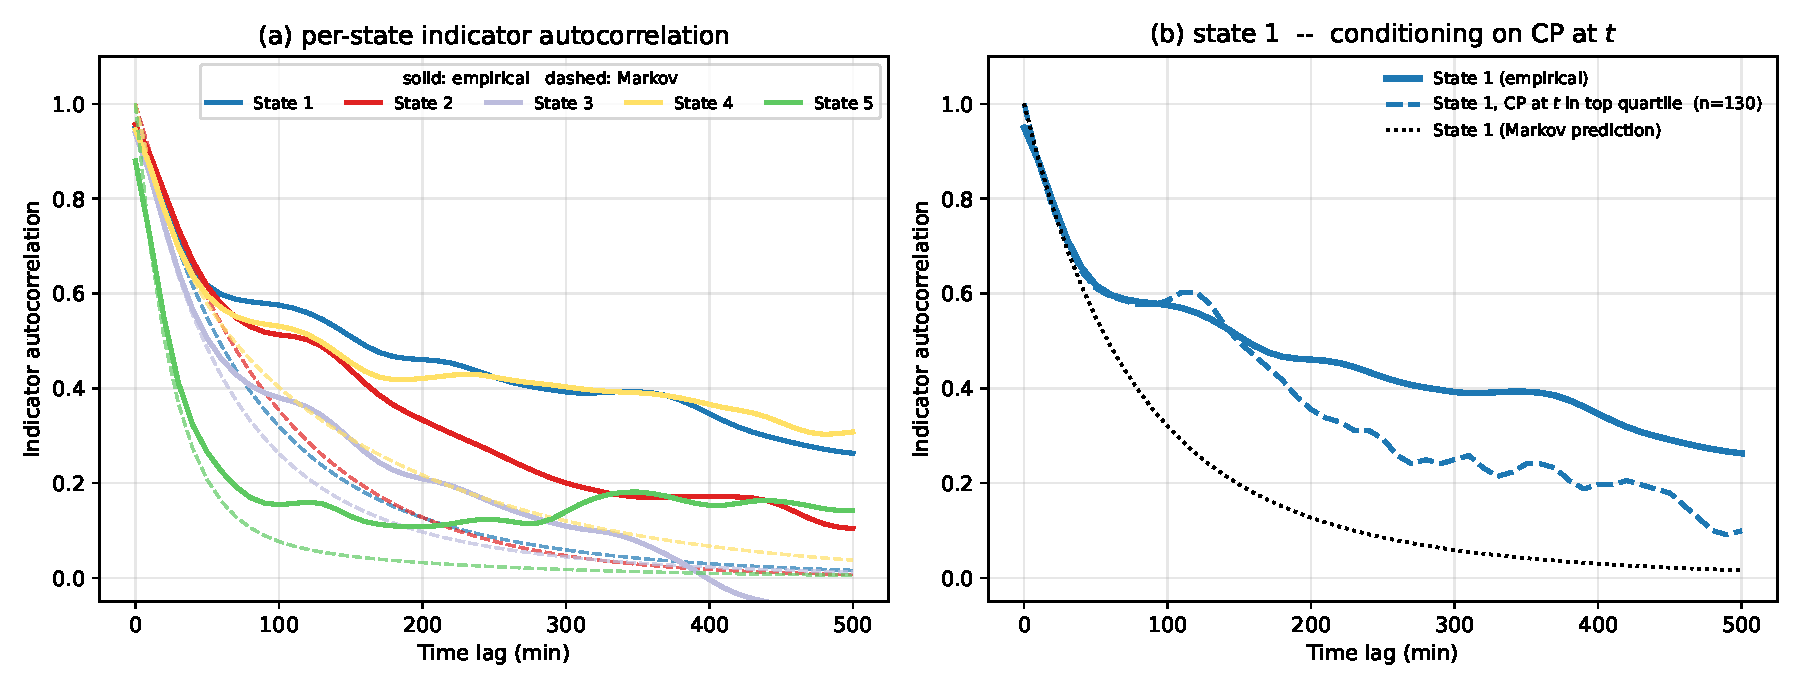
\includegraphics[width=0.9\textwidth]{fig9bis_markovianity_coldpools.pdf}
    \caption{\textbf{Markovianity assessment.} \textbf{(a)}~Per-state indicator autocorrelations (solid) and Markov predictions (dashed, same colour); states~1 and~4 sit above their predictions, the others track theirs. \textbf{(b)}~State-1 autocorrelation: empirical (solid), Markov prediction (dotted), and empirical conditioned on $\mathrm{CP}(t)>\mathrm{CP}_\star$ at the starting time (dashed), closing $\sim$30\% of the gap at a 200~min lag.}
    \label{fig:autocorrelation}
\end{figure*}

\section{Discussion}

Convection varies widely even under a fixed forcing, yet this variability is structured, not random. Casting the flow in isentropic coordinates and encoding it into a low-dimensional latent space, we reduced its evolution to a Markov chain over five discrete states that recover physically meaningful regimes. The chain is nearly memoryless: a single slow eigenmode ($\lambda_2\approx0.94$, $\tau_2\approx172$~min) alternates organized and unorganized regimes around a dominant suppressed background ($\pi_3=37\%$), with two competing routes---a direct ascent into deep convection and a slower drift through weakly organized phases. Its distinctive feature is diagnostic: departures from Markovianity reveal what the partition omits, and conditioning on cold-pool intensity closes $\sim$30\% of the gap at a $200$~min lag, identifying cold pools as one measurable carrier of the hidden memory.

These results describe a single idealized forcing, and the simplicity of the latent space may partly reflect that control. Because the transition matrix depends on the forcing, repeating the construction across shear regimes---weak (popcorn), moderate, strong (supercritical squall lines)---would turn convective organization into a measurable dynamical observable, with organized-state persistence $T_{ii}$ and eigenmode time scales lengthening under stronger shear.

\section*{Data and Code Availability}

The idealized squall-line SAM simulations (27 days at 2-minute resolution, with 1D, 2D, and 3D outputs) are available via Globus (link to be provided). All code is openly available at \url{https://github.com/sososquirrel/troposwhere}, including the model implementation and the scripts to reproduce all figures. Full methods---simulation setup, isentropic preprocessing, model architecture, training, and sensitivity tests---are given in the Supplemental Material.

\section*{Acknowledgments}

We are grateful to Juan Nathanael and Carla Roesch for discussions on Koopman operators, and to Fabrizio Falasca and Matthieu Blanke for recommendations on the dynamical systems literature. We also thank Sara Shamekh, Zhe Feng, Xingchao Chen, and the WACCEM project team for valuable discussions throughout the course of this study. We thank Koichi Sakaguchi and Huancui Hu for their internal review and constructive feedback. Portions of the manuscript were rephrased with the assistance of ChatGPT (OpenAI) for language editing, and Claude (Anthropic) assisted with aspects of code development and cleaning; all scientific ideas, analysis, and conclusions were developed by the authors. 

This study is supported by Office of Science, U.S. Department of Energy (DOE) Biological and Environmental Research as part of the Regional and Global Model Analysis program area through the Water Cycle: Modeling of Circulation, Convection, and Earth System Mechanisms (WACCEM) scientific focus area. S.A. designed the research, performed the simulations, developed the methods and code, and wrote the manuscript. O.P. contributed to the methodological development and the code and participated in the analysis and discussions. L.R.L. and P.G. contributed to improving the analysis and interpretation.

\bibliographystyle{apsrev4-2}
\bibliography{biblio}

\end{document}
